% !TeX root = ../Trabajo_RPM.tex
\subsection{Diseño reproducible de Monte Carlo}
El experimento utiliza la demanda diaria de 99 referencias como centro de perturbación. Para el escenario $s$ se genera un factor independiente por referencia y se aplica
\begin{equation}
D_i^{(s)}=\max\{1,\lfloor D_i\epsilon_i^{(s)}+0,5\rfloor\},\qquad
\epsilon_i^{(s)}\sim\mathcal U(0,85;1,15).
\end{equation}
La regla se encarga de mantener las cantidades enteras positivas y de redondear hacia arriba los casos con fracción 0,5. El generador histórico parte de una semilla 42. Al guardar los vectores que se generan se puede volver sobre el experimento sin tener que confiar en que una nueva versión de las bibliotecas sea capaz de reproducir cada detalle de la ejecución.

Se valora cada vector con una heurística y el modelo de asignación, empleando idéntica capacidad y tiempos. Para que la comparación tenga sentido es preciso que las dos soluciones den cobertura a toda la demanda. Un plan heurístico podría mostrar menos minutos si deja parte de la demanda sin atender, pero no sirve de base para medir el porcentaje de mejora del lote completo.

Los factores uniformes no se han estimado de un conjunto de pedidos, sino que son una ventana experimental de un 15\% alrededor de cada demanda nominal. La independencia supone que el experimento no representa correlaciones entre referencias derivadas de campañas, clientes o familias comerciales. Tales supuestos ponen un límite a la extrapolación, por mucho que el cálculo de los escenarios sea reproducible \cite{law}.

\subsection{Presupuesto de resolución y recuperación de resultados}
Con HiGHS se ha pedido una brecha relativa histórica de $10^{-4}$ (un 0,01\%) y un tiempo de cinco segundos por escenario. Para los tres casos en que no se hallaba un plan factible de comprobar a la primera se ha hecho un nuevo intento con treinta segundos. El expediente conserva tanto el resultado final como el primer intento. En el resumen figuran las mil comparaciones, no únicamente aquellas con un estado propicio.

Dicho presupuesto es del experimento de simulación, no del protocolo nominal de certificación posterior carente de límite interno; sin él no sería posible dar sentido a las brechas de la muestra. La calidad de los incumbentes está sujeta al criterio de detención, lo cual entra en la definición de la mejora que se observa.

En esta revisión se han traído de nuevo las mil filas de resultados y los vectores de demanda correspondientes. Se ha hecho cotejo de los identificadores, totales, fórmulas de mejora y estadísticos con el resumen de archivo. Las figuras se han generado de nuevo a partir de los CSV, sin embargo no se ha vuelto a ejecutar el MILP ni a convertir sus soluciones de antaño en nuevos certificados de optimalidad.

Los totales de la muestra van de 13.176 a 15.007 unidades de demanda. De los mil registros de cierre se infiere la factibilidad del MILP y que no hay faltantes en la heurística. Los mil planes que se conservan han sido reconstruidos; los residuos máximos de dominio, integralidad, enlace y demanda no superan $3,21\times10^{-9}$ y no existe exceso de capacidad. La divergencia más acusada entre el objetivo tal como fue registrado y el recalculado es de $5,46\times10^{-12}$ minutos. Pese a que todos están dentro de la tolerancia de $10^{-5}$, esta verificación no anula las brechas positivas.

\subsection{Resultados de mejora y dispersión}
Sea $E_s$ la carga de la heurística factible y $UB_s$ el objetivo del plan MILP disponible. Se calcula
\begin{equation}
R_s^{\mathrm{inc}}=100\left(1-\frac{UB_s}{E_s}\right).
\end{equation}
La media es 15,2\%, la mediana 15,2\% y la desviación estándar 0,7724 puntos porcentuales. Las mejoras observadas se sitúan entre 12,4763\% y 17,8972\%; las mil son positivas. Estas cifras describen la reducción de carga nominal frente a la regla comparada, no una reducción observada de costos de fabricación.

\begin{figure}[H]\centering
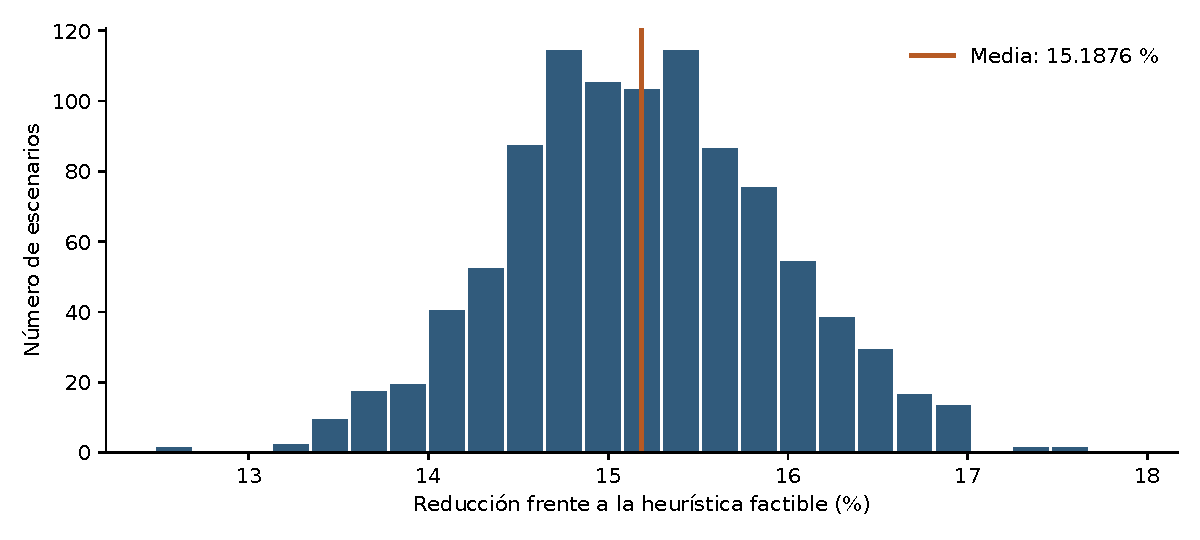
\includegraphics[width=\linewidth]{figuras/monte_carlo_mejora.pdf}
\caption{Distribución de la mejora de los incumbentes en los 1.000 escenarios históricos. La línea señala la media de la muestra.}
\fuente{recálculo a partir de \texttt{monte\_carlo\_escenarios.csv}; no corresponde a una nueva ejecución de los solvers}
\end{figure}

La concentración de la distribución no demuestra que toda demanda futura produzca una mejora semejante. Todos los escenarios provienen de una misma matriz nominal, una capacidad fija y una familia estrecha de perturbaciones. La dispersión observada combina variación del problema y calidad de las soluciones obtenidas dentro del presupuesto histórico.

La figura~\ref{fig:mcgap} permite inspeccionar la relación entre volumen y mejora, y la distribución de brechas. No se ajusta una ley causal entre volumen y rendimiento: los escenarios cambian simultáneamente las demandas de muchas referencias y, con ellas, la combinación de cargas y preparaciones.
\begin{figure}[H]\centering
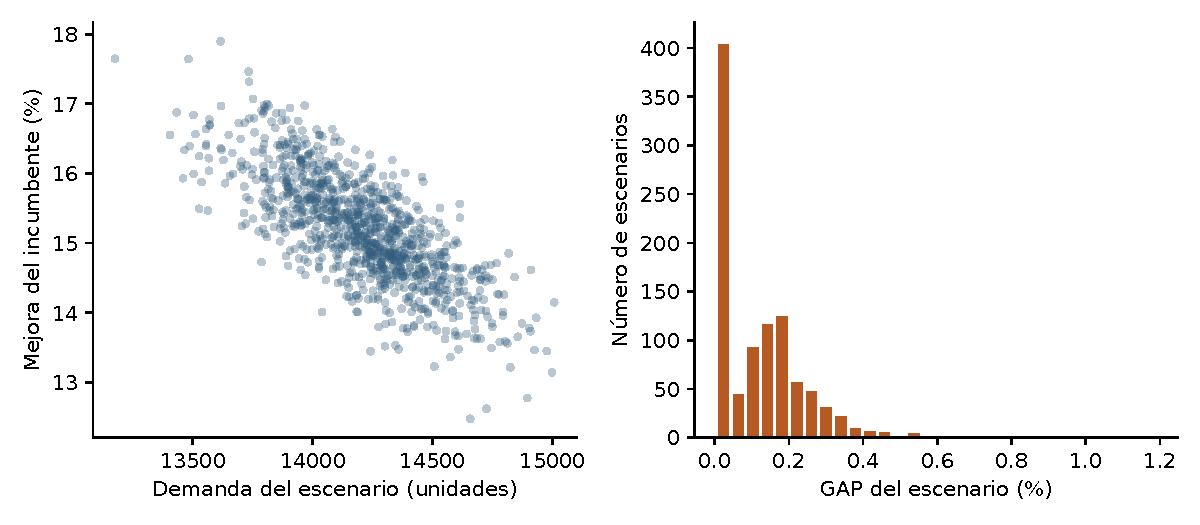
\includegraphics[width=\linewidth]{figuras/monte_carlo_gap.pdf}
\caption{Demanda respecto a mejoras y brechas finales de los escenarios. Cada punto representa una comparación factible.}\label{fig:mcgap}
\end{figure}

\subsection{Incertidumbre de muestreo e incertidumbre de optimización}
Si $LB_s\leq Z_s^*\leq UB_s$, la mejora frente a la heurística queda acotada por
\begin{equation}
100\left(1-\frac{UB_s}{E_s}\right)\leq R_s^*
\leq100\left(1-\frac{LB_s}{E_s}\right).
\end{equation}
La mejora que un plan factible ha logrado se sitúa en el extremo inferior. El extremo superior representa la mayor mejora compatible con la cota inferior del solver. En la muestra, el promedio de esos extremos se sitúa en [15,2\%; 15,3\%]. La incertidumbre residual de optimización con relación a la mejora media de los escenarios se cuantifica con una amplitud de 0,1043 puntos porcentuales.

Se ha anotado un GAP medio del 0,1229\% y uno máximo del 1,1879\%. Ningún escenario presenta un valor numéricamente nulo. Las cotas delimitan la mejora todavía posible, pero no permiten afirmar que el experimento haya certificado mil óptimos. Es una precaución que se une a un balance positivo: en todos los casos de la muestra los incumbentes factibles tienen ya una carga inferior a la heurística.

Un intervalo t de 95\% aproximado se mantiene para la media de las mejoras de los incumbentes:
\begin{equation}
\overline R\ \pm\ t_{0,975;999}\frac{s_R}{\sqrt{1000}}
=[15,1397\%;15,2355\%].
\end{equation}
Bajo el diseño de partida, este intervalo se debe a la variabilidad en la simulación. No tiene por objeto cubrir el error de imputación de los tiempos, las correlaciones que se hayan pasado por alto, las paradas reales o la mejora pendiente entre $UB$ y $LB$. De igual modo, no es un intervalo aplicable a cada escenario por su cuenta. Que coexista con las cotas de mejora no es contradictorio, pues son fuentes de incertidumbre distintas.

\subsection{Reoptimización frente a robustez de un plan fijo}
En cada escenario se puede modificar la asignación una vez que se conoce la demanda. Con el experimento se mide en qué medida la regla de planificación es capaz de adaptarse a las perturbaciones, no la resistencia de un plan nominal sin retoques. Si de lo que se tratara fuera de evaluar un plan fijo habría que ceñirse a las decisiones y cuantificar los excesos de capacidad, faltantes o acciones correctivas que se den en cada caso.

La optimización robusta da forma a unas decisiones amparadas contra conjuntos de incertidumbre, a cambio de un compromiso entre protección y el desempeño nominal \cite{bertsimas}. No se ha puesto en práctica ese procedimiento. La simulación de por sí es un análisis de sensibilidad reiterado y no cabe llamarla modelo robusto de modo automático por el hecho de haber contemplado mil demandas.

Para RPM, el resultado es una ventaja nominal consistente frente a la heurística dentro del diseño de simulación. Para pasar de ahí a una recomendación en condiciones de riesgo operativo harían falta distribuciones o conjuntos de incertidumbre con base en datos, un criterio de servicio y una política de reacción. Esta comparación muestra tales requisitos sin adjudicarles resultados que no se han calculado.
